\documentclass{beamer}

\usepackage[utf8]{inputenc}
\usecolortheme{beaver}
\usepackage{caption}
\usepackage{subcaption}
\usepackage{mathtools}
\usepackage{todonotes}
\usepackage{amsmath}
\usepackage{bm}
\usepackage{listings}
\usepackage{ragged2e}
\usepackage{fancyvrb}
\usepackage{titlecaps}

\Addlcwords{for a is but and with of in as the etc on to if}

\def\ci{\perp\!\!\!\!\!\perp}

\tikzstyle{latent} = [ draw, circle, inner sep = 2pt, minimum size = 0.65cm ]
\tikzstyle{observed} = [ draw, rectangle, inner sep = 2pt, minimum size = 0.65cm ]

\newtheorem{proposition}{Proposition}

\setbeamertemplate{section in toc}{\inserttocsectionnumber.~\inserttocsection}
\usetheme{Boadilla}
\makeatletter
\setbeamertemplate{footline}{%
    \leavevmode%
    \hbox{%
        \begin{beamercolorbox}[wd=.3\paperwidth,ht=2.25ex,dp=1ex,center]{author in head/foot}%
            \usebeamerfont{author in head/foot}\insertshortauthor\expandafter\beamer@ifempty\expandafter{\beamer@shortinstitute}{}{~~(\insertshortinstitute)}
        \end{beamercolorbox}%
        \begin{beamercolorbox}[wd=.55\paperwidth,ht=2.25ex,dp=1ex,center]{title in head/foot}%
            \usebeamerfont{title in head/foot}\insertshorttitle
        \end{beamercolorbox}%
        \begin{beamercolorbox}[wd=.15\paperwidth,ht=2.25ex,dp=1ex,right]{date in head/foot}%
            \usebeamerfont{date in head/foot}\insertshortdate{}\hspace*{2em}
            \insertframenumber{} / \inserttotalframenumber\hspace*{2ex} 
        \end{beamercolorbox}}%
        \vskip0pt%
    }
\makeatother

\begin{document}

\title[Combining Graphical and Algebraic Approaches for Identification in SEM]{Combining Graphical and Algebraic Approaches for Parameter Identification in Latent Variable Structural Equation Models}
\author [Ankan et. al.] {Ankur Ankan \inst{1} \and Inge Wortel \inst{1} \and Kenneth Bollen \inst{2} \and Johannes Textor \inst{1}}
\institute[]{\inst{1} Radboud University \and \inst{2} University of North Carolina}
\date{}
\maketitle

\begin{frame}
	\frametitle{\titlecap{Parameter identification}}
	\begin{block}{Identification}
		Given a DAG $ G = (V, E) $ and an observational dataset on $ V $, is the causal effect
		of $ \bm{X} \in V $ on $ Y \in V $ estimable?
	\end{block}
	\begin{figure}
		\centering
		\begin{subfigure}{0.5 \textwidth}
			\centering
			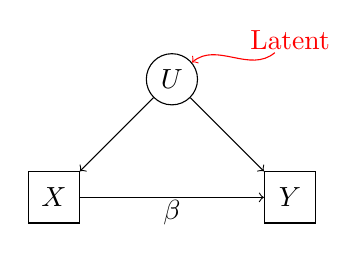
\begin{tikzpicture}
				\tikzstyle{every node}=[align=center, inner sep=1pt]
				\node[latent] (u) at (1.5, 1.5) {$ U $};
				\node[observed] (x) at (0, 0) {$ X $};
				\node[observed] (y) at (3, 0) {$ Y $};
				\node[text=red] (text) at (3, 2) {Latent};
				\draw[->] (u) -- (x);
				\draw[->] (u) -- (y);
				\draw[->] (x) -- (y) node[midway, below]{$ \beta $};
				\draw[->, red] (text) to [out=220, in=40] (u);
			\end{tikzpicture}
			\caption*{$ \beta $ is not identified}
		\end{subfigure}%
		\begin{subfigure}{0.5 \textwidth}
			\centering
			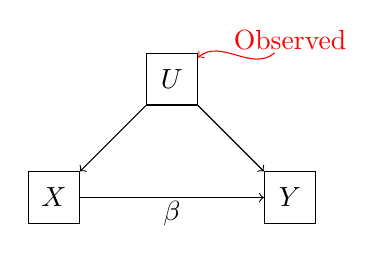
\begin{tikzpicture}
				\tikzstyle{every node}=[align=center, inner sep=1pt]
				\node[observed] (u) at (1.5, 1.5) {$ U $};
				\node[observed] (x) at (0, 0) {$ X $};
				\node[observed] (y) at (3, 0) {$ Y $};
				\node[text=red] (text) at (3, 2) {Observed};
				\draw[->] (u) -- (x);
				\draw[->] (u) -- (y);
				\draw[->] (x) -- (y) node[midway, below]{$ \beta $};
				\draw[->, red] (text) to [out=220, in=40] (u);
			\end{tikzpicture}
			\caption*{$ \beta $ is identified}
		\end{subfigure}
	\end{figure}
	\begin{itemize}
		\item \justifying{Pearl's do-calculus provides a complete solution for identification in non-parametric models.}
		\item \justifying{No practical general algorithm exists.}
		\item \justifying{Criteria like back-door, front-door, intrumental sets, etc. provide convenient solutions in special cases.}
	\end{itemize}
\end{frame}

\begin{frame}
	\frametitle{\titlecap{Instrumental Variables(IV)}}

	\begin{block}{Instrumental Variable}
		A variable $ Z $ qualifies as instrumental, relative to a cause $ X $ and effect $ Y $ if:
		\begin{enumerate}
			\item $ Z $ is independent of all error terms that have an influence on $ Y $ which is not mediated by $ X $
			\item $ Z $ is not independent of $ X $.
		\end{enumerate}
	\end{block}
	\begin{figure}
		\centering
		\begin{subfigure}{0.5\linewidth}
			\centering
			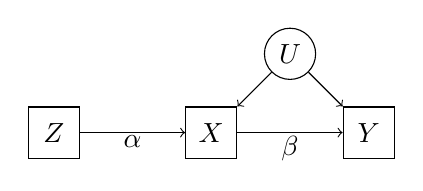
\begin{tikzpicture}
				\tikzstyle{every node}=[align=center, inner sep=1pt]
				\node[observed] (z) at (0, 0) {$ Z $};
				\node[observed] (x) at (2, 0) {$ X $};
				\node[observed] (y) at (4, 0) {$ Y $};
				\node[latent] (u) at (3, 1) {$ U $};
				\draw[->] (z) -- (x) node[midway, below] {$ \alpha $};
				\draw[->] (x) -- (y) node[midway, below] {$ \beta $};
				\draw[->] (u) -- (x);
				\draw[->] (u) -- (y);
			\end{tikzpicture}
			\caption{}
		\end{subfigure}%
		\begin{subfigure}{0.5\linewidth}
			\centering
			$$ \beta = \frac{Cov(Y, Z)}{Cov(Z, X)} = \frac{\alpha \beta}{\alpha}$$
			\caption{}
		\end{subfigure}
		\caption*{\centering{(a) $ Z $ is an IV for estimating $ \beta $ (b) Estimating $ \beta $ from observational data using $ Z $ as an IV.}}
	\end{figure}
\end{frame}

\begin{frame}
	\frametitle{\titlecap{IV Based Identification Criterion for Directed Acyclic Graphs (DAGs)}}
	\begin{itemize}
		\item In more complicated cases where the variables $ X $ and $ Y $ are sets we need to be more careful.
			\todo[inline]{Add an example of more complicated example here}
		\item Well studied problem and few identification criteria have been proposed.
		\item Examples are Instrumental Set (Brito and Pearl 2022), Instrumental Cutsets, Auxiliary Variables.
	\end{itemize}
	\todo[inline]{Add references here}
	% \begin{block}{Instrumental Set Criterion (Brito and Pearl 2002)}
	% 	Given an ADMG $\cal G$, a variable $y$, and a subset $X$ of the
	% 	parents of $y$,  a set of variables $I$ fulfills the
	% 	\emph{instrumental set condition} if for {some} permutation $
	% 	i_1 \ldots i_k $ of $ I $ and {some} permutation $ x_1 \ldots
	% 	x_k $ of $ X $ we have: 
	% \begin{enumerate}
	% 	\item There are no treks from $I$ to $y$ in the graph ${\cal
	% 		G}_{\overline{X}}$ obtained by removing all arrows
	% 		between $X$ and $y$. 
	% 	\item For each $j$, $1 \leq j \leq k$, there is a trek $\pi_j$ from
	% 		$I_j$ to $X_j$ such that for all $i < j$: (1) $I_i$ does not
	% 		occur on any trek $\pi_j$; and (2) all intersections between
	% 		$\pi_i$ and $\pi_j$ are on the left side of $\pi_i$ and the
	% 		right side of $\pi_j$.
	% \end{enumerate}
	% \end{block}
\end{frame}

\begin{frame}
	\frametitle{\titlecap{IV Based criterion for Structural Equation Models (SEMs)}}
		\begin{itemize}
		\item The IV criteria developed for DAGs always assume that the effect being estimated is between two observed variables.
		\item These criteria cannot be directly applied to SEMs as they usually have a latent level and observed measurement variables.
		\item Model Implied Instrumental Variables (MIIV) is a criterion for SEMs.
		\item Main idea behind MIIV is to replace latent variables with observed variables by doing a Latent-to-Observed (L2O) transformation.
	\end{itemize}
\begin{figure}
	\centering
	\includegraphics[page=1]{figures-inge.pdf}
	\caption{\footnotesize SEM based on the \emph{Industrialization and
		 Political Democracy} model with latent
		 variables $ l_1 $ (industrialization), and $ l_2 $ (political democracy).
		 The model contains 3 indicators for $ l_1 $: (1) gross
		 national product ($ y_1 $), (2) energy consumption
		 ($ y_2 $), and (3) labor force in industry ($ y_3 $), and 4
		 indicators for $ l_2 $: (1) press freedom rating ($y_4$), (2)
		 political opposition freedom ($y_5$), (3) election fairness
		 ($y_6$), and (3) legislature effectiveness ($y_7$). $
		 \lambda_{11} \dots \lambda_{13}, \lambda_{24} \dots
		 \lambda_{27}, \text{ and } \beta_{11} $ are the path
		 coefficients. $ \epsilon_1, \dots, \epsilon_7, \text{ and }
		 \zeta_1 $ represent noise/errors.}
	\label{fig:example_sem}
\end{figure}
\end{frame}

\begin{frame}
	\frametitle{\titlecap{Contributions}}
	\begin{figure}
		\centering
		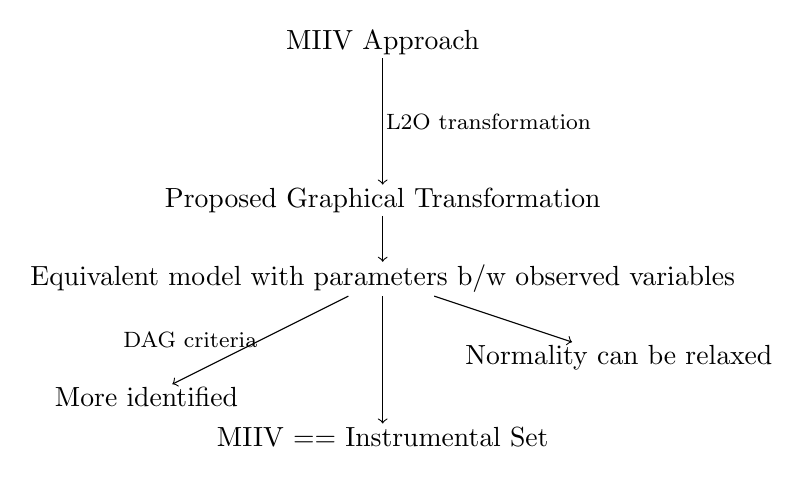
\begin{tikzpicture}
			\tikzstyle{every node}=[align=center, inner sep=1pt]
			\node (miiv) at (0, 0)  {MIIV Approach};
			\node (graphical) at (0, -2) {Proposed Graphical Transformation};
			\node (equivalent) at (0, -3) {Equivalent model with parameters b/w observed variables};
			\node (moreiden) at (-3, -4.5) {More identified};
			\node (equiproof) at (0, -5) {MIIV == Instrumental Set};
			\node (relax) at (3, -4) {Normality can be relaxed};
			
			\draw[->](miiv.south) to node[right] {\footnotesize L2O transformation} (graphical.north);
			\draw[->](graphical) -- (equivalent);
			\draw[->](equivalent) to node[left] {\footnotesize DAG criteria} (moreiden);
			\draw[->](equivalent) -- (equiproof);
			\draw[->](equivalent) -- (relax);


			% \node[tikztext] (ivdag) at (6, 2) {IV criteria for \\ graphical models};
			% \node[tikztext] (ivsem) at (0, 0) {IV iden. \\ in SEM};
			% \node[tikztext] (graphl2o) at (3, 0) {Graphical L2O \\ transform};
			% \node[tikztext] (graphidden) at (6, 0) {Graphical iden. \\ for SEM};
			% \node[tikztext] (graphcri) at (9, 3) {Can apply any \\ graphical criteria \\ to SEMs};
			% \node[tikztext] (equival) at (9, 0) {Equivalence proof};
			% \node[tikztext] (normal) at (9, -3) {Relaxing normality \\ condition}; 
			% \draw[->] (ivsem) -- (graphl2o);
			% \draw[->] (ivdag) -- (graphidden);
			% \draw[->] (graphl2o) -- (graphidden);
			% \draw[->] (graphidden) -- (graphcri);
			% \draw[->] (graphidden) -- (equival);
			% \draw[->] (graphidden) -- (normal);
		\end{tikzpicture}
	\end{figure}
\end{frame}

\begin{frame}
	\frametitle{\titlecap{SEM and Latent-to-Observed (L2O) Transformation}}
	\begin{equation}
		\begin{split}
			X &= \mathbf{B} X + E \\
			x_i &= \epsilon_i + \sum_{x_j \in Co(x_i)}\beta_{x_j \rightarrow x_i} x_j \\
			x_i &= \epsilon_i + \sum_{x_j \in Co_l(x_i)} \beta_{x_j \rightarrow x_i} (x_j^s - \epsilon_{x_j^s}) + \sum_{x_k \in Co_o(x_i)} \beta_{x_k \rightarrow x_i} x_k
		\end{split}
	\end{equation}
	

\end{frame}

\begin{frame}
	\frametitle{\titlecap{Proposed graphical transformation: Latent $ \rightarrow $ Observed}}
	\begin{figure}
		\centering
		\includegraphics[page=4]{figures-inge.pdf}
		\caption{}
		\label{fig:l2o_parent}
	\end{figure}
\end{frame}
\begin{frame}
	\frametitle{\titlecap{Proposed graphical transformation: Observed $ \rightarrow $ Latent}}
	\begin{figure}
		\centering
		\includegraphics[page=5]{figures-inge.pdf}
		\caption{}
		\label{fig:l2o_child}
	\end{figure}
\end{frame}
\begin{frame}
	\frametitle{\titlecap{Proposed graphical transformation: Latent $ \rightarrow $ Latent}}
	\begin{figure}
		\centering
		\includegraphics[page=6]{figures-inge.pdf}
		\caption{}
		\label{fig:l2o_both}
	\end{figure}
\end{frame}

\begin{frame}
	\frametitle{\titlecap{Identification Examples: Full Equations}}
		\begin{figure}[t]
			\begin{subfigure}[b]{0.5 \linewidth}
				\centering
				\includegraphics[page=7]{figures-inge.pdf}
				\caption{}
				\label{fig:transform_example}
			\end{subfigure}%
			\begin{subfigure}[b]{0.5 \linewidth}
				\centering
				\includegraphics[page=8]{figures-inge.pdf}
				\caption{}
				\label{fig:transform_example_single}
			\end{subfigure}
		\caption{(a) Example model following the structure of
			Figure~\ref{fig:example_sem} with explicit error terms. 
			(b) L2O transformation for the model in (a) for identifying both
			coefficients of the equation for $y_3$ simultaneously. We end up with
			the regression equation $y_3 \sim y_2 + y_4$ and can identify both
			coefficients using $y_1$ and $y_5$ as instrumental variables.}
		\label{fig:examples1}
		\end{figure}
\end{frame}

\begin{frame}
	\frametitle{\titlecap{Identification Examples: Partial Equations}}
		\begin{figure}[t]
			\centering
			\begin{subfigure}[b]{0.33 \linewidth}
				\centering
				\includegraphics[page=11]{figures-inge.pdf}
				\caption{}
				\label{fig:example_orig}
			\end{subfigure}%
			\begin{subfigure}[b]{0.33 \linewidth}
				\centering
				\includegraphics[page=12]{figures-inge.pdf}
				\caption{}
				\label{fig:example_non_corr}
			\end{subfigure}%
			\begin{subfigure}[b]{0.33 \linewidth}
				\centering
				\includegraphics[page=13]{figures-inge.pdf}
				\caption{}
				\label{fig:transform_non_corr}
			\end{subfigure}
			\caption{(a) Adapted SEM from; modified by making $ l_1
				 $ and $ l_2 $ uncorrelated and $ \epsilon_1 $ and $ \epsilon_2
				 $ correlated. (b) Transformed model for estimating $ y_3 \sim
				 l_1 + l_2 $. The equation is not identified as $ y_5 $ is the
				 only IV. (c) With partial L2O transformation, $ \lambda_{23} $
				 can be estimated using $ y_5 $ as the IV.}
		\label{fig:examples3}
		\end{figure}
\end{frame}

\begin{frame}
	\frametitle{\titlecap{More Identification: Conditional IVs}}
	\begin{figure}[t]
		\centering
		\begin{subfigure}[b]{0.5 \linewidth}
			\centering
			\includegraphics[page=14]{figures-inge.pdf}
			\caption{}
			\label{fig:example_conditional_iv}
		\end{subfigure}%
		\begin{subfigure}[b]{0.5 \linewidth}
			\centering
			\includegraphics[page=15]{figures-inge.pdf}
			\caption{}
			\label{fig:transform_conditional_iv}
		\end{subfigure}
		\caption{(a) Modified version of the Figure~\ref{fig:example_orig} model, where $l_1$ and $l_2$
			share an observed cause $y_6$.
			$\lambda_{13} $ and $ \lambda_{23} $ are still not
			simultaneously identified as no IVs are available. (b) Even
			with partial transformation, $ \lambda_{23} $ is no longer
			identified as $ y_5 $ is not an IV because of the open paths $
			y_5 \gets l_2 \gets y_6 \to y_3 $ and $ y_5 \gets l_2 \gets y_6
			\to l_1 \to y_3 $. However, using the conditional instrumental
			set criterion, we can identify $\lambda_{23}$ by using $y_5$ as
			a \emph{conditional IV} for the equation $y_3 \sim y_4$, as
			conditioning on $ y_6 $ blocks the open paths.}
	\label{fig:examples4}
	\end{figure}
\end{frame}

\begin{frame}
	\frametitle{\titlecap{Example: Identified but not estimable}}
\begin{figure}[t]
	\centering
	\begin{subfigure}[b]{0.33 \linewidth}
		\centering
		\includegraphics[page=16]{figures-inge.pdf}
		\caption{}
		\label{fig:example_original_model}
	\end{subfigure}%
	\begin{subfigure}[b]{0.33 \linewidth}
		\centering
		\includegraphics[page=17]{figures-inge.pdf}
		\caption{}
		\label{fig:example_incorrect_estimate}
	\end{subfigure}%
	\begin{subfigure}[b]{0.33 \linewidth}
		\centering
		\includegraphics[page=18]{figures-inge.pdf}
		\caption{}
		\label{fig:transform_incorrect_estimate}
	\end{subfigure}%
	\caption{(a) An example model from 
	about the economic effects of schooling. The model has $ 1 $ latent
	variable $x_1$ (Ability) with $ 4 $ observed variables $ y_1 $ (IQ), $
	y_2 $ (Schooling), $ y_3 $ (knowing how the world works), and $ y_4 $
	(Income). (b) A slightly modified version of the model in
	Figure~\ref{fig:example_original_model} where we add two new edges $ y_1
	\rightarrow y_2 $ and $ y_3 \rightarrow y_4 $.  (c) L2O transformed
	model for the equation of $ y_4 $. The transformed regression equation
	for $ y_4 $ is: $ y_4 \sim y_3 + y_2 $ but because of the
	transformation, the coefficient of $ y_3 $ has changed
	to $ \lambda_{14} + \lambda_{34} $. Because of this changed
	coefficient, even though the equation is identified, it is not possible
	to estimate either $ \lambda_{14} $ or $ \lambda_{34} $ individually.
	}
\label{fig:examples5}
\end{figure}
\end{frame}

\begin{frame}
	\frametitle{\titlecap{Instrumental Set and Algebraic Instrumental Set are Equivalent}}
		\begin{definition}[Permutation-free Instrumental Sets]
		\label{defn:graphicistrek}
			Given an ADMG $\cal G$, a variable $y$ and a subset $X$ of the parents
			of $y$, a set of variables $I$ fulfills the \emph{permutation-free
			instrumental set condition} if: (1) There are no treks from $I$ to $y$
			in the graph ${\cal G}_{\overline{X}}$ obtained by removing all arrows
			leaving $X$, and (2) All $t$-separators $(L,R)$ of $I$ and $X$ have
			size $\geq k$. 
		\end{definition}

		\begin{definition}[Algebraic Instrumental Sets]
			\label{defn:algebraicis}
			Given a regression equation $y = B \cdot X + \epsilon$, where $X$ possibly
			correlates with $\epsilon$, a set of variables
			$I$ fulfills the \emph{algebraic instrumental set condition} if: (1) $I \ci \epsilon$,
			(2) $\textrm{rk}(\bm{\Sigma}[I,X]) = |X|$, and (3) $\textrm{rk}(\bm{\Sigma}[I]) = |I|$
		\end{definition}
\end{frame}

\begin{frame}
	\frametitle{\titlecap{Conclusion}}
	\begin{itemize}
		\item We propose a graphical L2O tranform similar to the algebraic L2O transform used in MIIV approach.
		\item The graphical transformation allows to use the graphical IV criteria on latent varialbe SEM.
		\item We show that the graphical instrumental set criterion is equivalent to the algebraic criterion.
		\item The application of graphical IV criteria leads to identification of more parameters in SEMs.
		\item The SEM literature is more developed than the graphical
			literation when it comes to non-Gaussian models. For
			example, MIIV with two-stages least squares estimation
			is asymptotically distribution-free, and our results
			imply that normality is not required for applying the
			instrumental set criterion.
	\end{itemize}
\end{frame}
\end{document}
